\documentclass[twoside]{article}

\usepackage[a4paper, total={674pt, 426pt}, landscape]{geometry}
\usepackage{multicol}

\newcommand{\todo}[1]{\textcolor{red}{\textbf{TODO:} #1}}
\newcommand{\dyade}[1]{\overleftrightarrow{#1}}
\newenvironment{definition}[1]{\begin{tcolorbox}[title=Def.: #1, colback=white!,colframe=green!50!black]}{\end{tcolorbox}}

\titlespacing*{\section}{0pt}{.6\baselineskip}{.1\baselineskip}
\titlespacing*{\subsection}{0pt}{.6\baselineskip}{.1\baselineskip}
\titlespacing*{\subsubsection}{0pt}{.6\baselineskip}{.1\baselineskip}


%% This is the space for custom commands for your Formelsammlung
\newcommand{\FormelsammlungTitel}{Technische Felder und Wellen}
\newcommand{\FormelsammlungAutor}{Bogdan Stamenic}
\setcounter{tocdepth}{2} % Show only sections and subsection in table of contents

\begin{document}
	\title{\FormelsammlungTitel}
	\author{\FormelsammlungAutor}
	\date{\today}
    \begin{multicols}{3}
                \maketitle
        \tableofcontents
		\section{Grundlagen}
		\subsection{Mathematik}
		\subsubsection{Mehrdimensionale Integrale}
		\begin{center}
			\textbf{Kurvenintegrale:}\\%
			\begin{align*}
				\int\limits_{\mathcal{C}}f(\vec{r})\mathrm{d}s &= \int\limits_a^b\ f(\vec{r}(t))\,|\vec{r^{\prime}}(t)|\mathrm{d}t;\
				\quad \vec{r}:[a,b]\to\mathcal{C}\\
				\int\limits_{\mathcal{C}}\vec{F}(\vec{r})\mathrm{d}s &= \int\limits_a^b\ \vec{F}(\vec{r}(t))\cdot\vec{r^{\prime}}(t)\mathrm{d}t;\
				\quad \vec{r}:[a,b]\to\mathcal{C}\\
			\end{align*}
			\textbf{Oberflächenintegrale:}
			\begin{align*}
				\iint\limits_A f \mathrm{d}\vec{a} &= \iint\limits_A f(\vec{x}(s,t))\!\
				\left\|\dfrac{\partial\vec{x}}{\partial s}\times\dfrac{\partial\vec{x}}{\partial t}\right\|\
				\mathrm{d}s\mathrm{d}t\\
				\iint\limits_A \vec{F} \mathrm{d}\vec{a} &= \iint\limits_A \vec{F}(\vec{x}(s,t))\cdot\!\
				\left( \dfrac{\partial\vec{x}}{\partial s}\times\dfrac{\partial\vec{x}}{\partial t} \right)\
				\!\mathrm{d}s\mathrm{d}t\\
			\end{align*}
			\textbf{Volumenintegrale:}
			\begin{align*}
				V &= \iiint\limits_V f(x,y,z)\:\mathrm{d}x\mathrm{d}y\mathrm{d}z\\
				&= \iiint\limits_V f(\rho,\varphi,z)\,\rho\:\mathrm{d}\rho\mathrm{d}\varphi\mathrm{d}z\\
				&= \iiint\limits_V f(r,\varphi,\theta)\,r^2\sin\theta\:\mathrm{d}r\mathrm{d}\varphi\mathrm{d}\theta\\
			\end{align*}
		\end{center}
        \subsubsection{Integraltheoreme}
        \textbf{Integralsatz von Gauß:}
            \[\iiint\limits_V \mathrm{div}\:\vec{a}\,\mathrm{d}v = \oiint\limits_{A(V)} \vec{a}\,\mathrm{d}\vec{A}\]
        \subsubsection{Vektoralgebra}
        %\(\vec{a}\times\vec{b} = -\vec{b}\times\vec{a}\)
        \textbf{Spatprodukt:}\\
        \[(\vec{a} \times \vec{b}) \cdot \vec{c} = (\vec{c} \times \vec{a}) \cdot \vec{b}\]\\
	 \subsection{Maxwell-Gleichungen}
	 \subsubsection{Integralform}
		{\small%
		\begin{flalign*}
			& \mathrm{\textbf{Gauß'sche Gesetz:}}\\
			& \oiint\limits_{A(V)}\vec{D}_m\cdot\mathrm{d}\vec{A} = \iiint\limits_V\rho\mathrm{d}V = Q\\
			& \mathrm{\textbf{Magnetische Quellenfreiheit:}}\\
			& \oiint\limits_{A(V)}\vec{b}\cdot\mathrm{d}\vec{A} = 0\\
			& \mathrm{\textbf{Induktionsgesetz:}}\\
			& \oint\limits_C\vec{e}\cdot\mathrm{d}\vec{s} =%
			-\dfrac{\mathrm{d}}{\mathrm{d}\vec{t}}\iint\limits_A\vec{b}\cdot\mathrm{d}\vec{A} = -\dfrac{\mathrm{d}\Phi_m}{\mathrm{d}t}\\
			& \mathrm{\textbf{Durchflutungsgesetz:}}\\
			& \oint\limits_C\vec{h}\cdot\mathrm{d}\vec{s} = \iint\limits_A\left[\vec{j}+\dfrac{\mathrm{d}\vec{D}_m}{\mathrm{d}t}\right]\cdot\mathrm{d}\vec{A} = i_{ges}\\
		\end{flalign*}
		}
	 \subsubsection{(Zeitfreie) Differentielle Form}
	 {\small%
	 \begin{align*}
	  &\mathrm{\textbf{Differentiell}} & \mathrm{\textbf{Zeitfrei (harm. Wellen)}}\\
	 	&\nabla\times\vec{e} = -\dfrac{\partial\vec{b}}{\vec{\partial t}} & \nabla\times\vec{E} = -j\omega\vec{B}\\
	 	&\nabla\times\vec{h} = \vec{j} +\dfrac{\partial\vec{D}_m}{\vec{\partial t}} & \nabla\times\vec{H} = \vec{J} + j\omega\vec{D}_m\\
		&\nabla\cdot\vec{D}_m = \rho & \nabla\cdot\vec{D}_m = \rho\\
		&\nabla\cdot\vec{b} = \rho_m & \nabla\cdot\vec{B} = \rho_m
	 \end{align*}
	 }
	 \subsubsection{Kontinuitätsgleichung des Stroms}
	 {\small%
	 \begin{align*}
	 	& \mathrm{\textbf{Integrale Form}}\\
		& \oint\limits_{A(V)}\vec{j}\cdot\mathrm{d}\vec{A} = -\int\limits_v \dfrac{\partial \rho}{\partial t} \mathrm{d}v\\
		& \mathrm{\textbf{Differentielle Form}}\\
		& \nabla\cdot\vec{j} = -\dfrac{\partial \rho}{\partial t}\\
		& \mathrm{\textbf{Zeitfreie Form}}\\
		& \nabla\cdot\vec{J} = -j\omega\rho
	 \end{align*}
	 \subsubsection{Entkopplung der Maxwell-Gleichungen}
	 \begin{itemize}
	 	\itemsep0pt
		\item Differentielle Maxwell-Gleichungen
		\item \(\epsilon_r, \mu_r = \mathrm{konst.}\)
		\item \(\kappa = 0, \vec{J} \neq 0\)\\
	 	\(\implies\) \textbf{Wellengleichung:}\\\vspace{2pt}
		\(\nabla\!\times\!\nabla\!\times\!\vec{E} - k^2\vec{E} = -j\omega\mu_r\mu_0\vec{J}\)
		\item Quellenfrei \(\vec{J} = 0\)
		\item \(\nabla\!\times\!\nabla\!\times\!\vec{F} = \mathrm{grad}\;\mathrm{div}\vec{F} - \Delta\vec{F}\)\\
		\(\implies\) \textbf{Helmholtz-Gleichung:} \(\Delta\vec{E} + k^2\vec{E} = 0\)
	 \end{itemize}

	 \subsubsection{Rand- und Stetigkeitsbedingungen}
	 \begin{itemize}
	 	\itemsep0pt
		\item \textbf{Tangentialkomponenten}
		\begin{itemize}
			\itemsep0pt
			\item Normalfall: \(\vec{n}\times\left(\vec{h}_1 - \vec{h}_2\right) = 0\)
			\item Oberflächenströme: \(\vec{n}\times\left(\vec{h}_1 - \vec{h}_2\right) = \vec{j}_F\)
			\item \(\vec{n}\times\left(\vec{e}_1 - \vec{e}_2\right) = 0\)
		\end{itemize}
		\item \textbf{Normalkomponenten}
		\begin{itemize}
			\itemsep0pt
			\item Normalfall: \(\vec{n}\cdot\left(\vec{D}_{m1} - \vec{D}_{m2}\right) = 0\)
			\item Oberflächenladungen: \(\vec{n}\cdot\left(\vec{D}_{m1} - \vec{D}_{m2}\right) = \rho_F\)
			\item \(\vec{n}\cdot\left(\vec{b}_1 - \vec{b}_2\right) = 0\)
		\end{itemize}
	 \end{itemize}
	 }

	 \subsection{Skin-Effekt}%
	 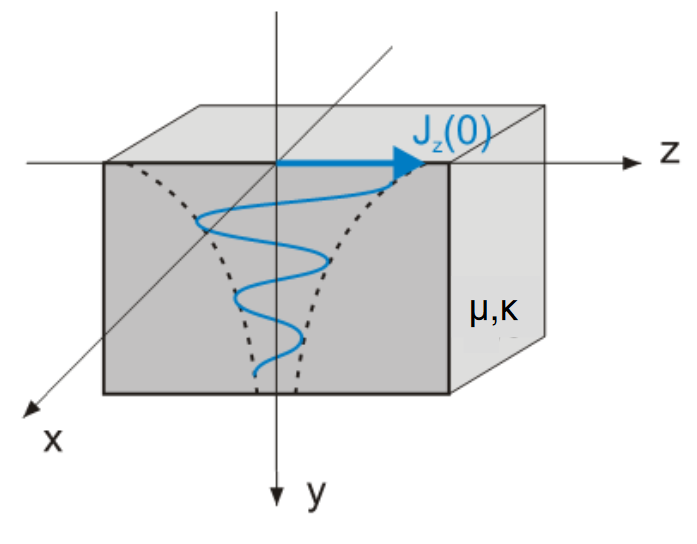
\includegraphics[width=.3\paperheight]{content/fuw/pictures/skin_effect.png}
	 {\small%
	 \begin{itemize}
	 	\itemsep0pt
		\item ideale Leiter \(\kappa\to\infty:\: E_{tan} = 0\)\\
		\(\implies\) nur in einer infitesimal dünnen Schicht existieren Oberflächenströme
		\item guter Leiter \(\kappa\gg\omega\epsilon\), verlustbehaftet:
		\begin{itemize}
			\itemsep0pt
			\item in einer dünnen Schicht unter der Oberfläche existieren nennenswerte Stromdichten\\
			\item Für die Verluste sind nur die obersten Schichten des Leiters entscheidend
			\item \textbf{Stromverteilung im Leiter:}\\
			\(J_z = J_z(0)e^{-ky}e^{-jky};\;\;k=\sqrt{\dfrac{\omega\mu\kappa}{2}}\)\\
			\(\implies \mathrm{\textbf{Eindringtiefe:}}\;\; \delta = \dfrac{1}{k} = \sqrt{\dfrac{2}{\omega\mu\kappa}}\)
		\end{itemize}
		\item Joule'sche Verluste: \(P_J = \frac{1}{2}\int\limits_S R_S |H_0|^2\mathrm{d}A\)\\
		\(\implies\) \textbf{Oberflächenimpedanz:}\\
		\(Z_S = R_S (1 + j) = (1 + j)\sqrt{\dfrac{\omega\mu}{2\kappa}}\)
	 \end{itemize}
	 }

	 \subsection{Ebene Wellen}
	 {\small%
	 \subsubsection{Ebene Wellen mit Ausbreitung in z-Richtung}
	 \begin{enumerate}
	 	\itemsep0pt
		\item Gute Approximation für reale Wellen \(\to\) Fernfelder von Antennen als lokal ebene Wellen
		\item Darstellung beliebiger Wellenfelder als Überlagerung ebener Wellen \(\to\) Fourier-Transformation
		\item Einfach handhabbar, z.B. bei Einfall auf ebene Grenzflächen
	 \end{enumerate}
	 \begin{itemize}
	 	\itemsep0pt
		\item Phasenfronten sind Ebenen
		\item Wellenvektor \(\vec{k}\) ist normal zu den Ebenen
		\item Ausbreitung in z-Richtung: \(\frac{\partial}{\partial x} = \frac{\partial}{\partial y} = 0\)
		\item (stückweise) homogenes, lineares Medium: \(\mu, \epsilon = \mathrm{const.}\)
		\item keine freie Ladungen: \(\rho = 0\)
		\item verschwindende Leitfähigkeit: \(\kappa = 0\)\\
		\(\implies\) Symmetrie, d.h. Lösung für E-Feld \textit{oder} H-Feld genügt
		\item ist eine \textbf{TEM-Welle} (nicht-dispersiv, keine longitudinale Komponente)
		\item 1D-Helmholtz-Gleichung: \(\dfrac{\partial^2e_x}{\partial z^2} - \epsilon\mu \dfrac{\partial^2 e_x}{\partial t^2} = 0\)\\
		\(\implies\) Lösung:\\
		\(e_x(z,t) = E_1 f_1\left(t - \dfrac{z}{c}\right) + E_2 f_2\left(t + \dfrac{z}{c}\right)\)\\
		\(\implies\) Ausbreitungsgeschwindigkeit: \(c = \dfrac{1}{\sqrt{\epsilon\mu}}\)
		\item \(e_x(z,t) = \sqrt{\dfrac{\mu}{\epsilon}} h_y(z,t) = Z_F\, h_y(z,t) \)\\
		\(\implies\) \textbf{Wellenwiderstand des Vakuums:}\\
		\(Z_{F_0} = \sqrt{\dfrac{\mu_0}{\epsilon_0}} \approx 120\pi\,\Omega \approx 377\,\Omega\)
	 \end{itemize}
	 \subsubsection{Harmonische Ebene Wellen}
	 \begin{flalign*}
	 	e_x(z,t) &= E \cos\left[\omega\left(t - \dfrac{z}{c}\right)\right]\\
		h_y(z,t) &= \dfrac{E}{Z_F} \cos\left[\omega\left(t - \dfrac{z}{c}\right)\right]
	 \end{flalign*}
	 \begin{itemize}
	 	\itemsep0pt
		\item Periodenabstand/Wellenlänge:\\
		\(\lambda = \dfrac{2\pi c}{\omega} = \dfrac{c}{f}\)
		\item \textbf{Phasenkonstante \(\beta\):}\\
		\(\beta = \dfrac{\omega}{c} = \dfrac{2\pi}{\lambda}\)
		\item zeitfreie Gleichungen:\\\smallskip
		\(E_x(z,t) = \mathrm{Re}\left\{E_x(z)e^{j\omega t}\right\}\)\\
		\(\implies E_x(z) = E e^{-j\beta z}\)\\
		\(\implies H_y(z) = \dfrac{E}{Z_F} e^{-j\beta z}\)
	 \end{itemize}
	 \subsubsection{Polarisation Ebener Wellen}
	 % TODO: Add screenshot with from Polarization slide
	 \subsubsection{Phasen-/Gruppengeschwindigkeit}
	 \begin{itemize}
	 	\itemsep0pt
		\item \textbf{Dispersionsfreiheit} \(\implies v_{ph} = \dfrac{\omega}{\beta} = v_g\)
		\item Wellenlänge (Phasengeschwindigkeit) frequenzabhängig \(\to\) Frequenzkomponenten eines Signals breiten sich unterschiedlich schnell aus
		\item die Ausbreitungsgeschwindigkeit der Modulation bezeichnet man als \textbf{Gruppengeschwindigkeit:}\\\smallskip
		\(v_g = \dfrac{1}{\Delta\beta / \Delta\omega} \;\implies v_g = \left(\dfrac{\mathrm{d}\beta}{\mathrm{d}\omega}\right)^{-1}\)
	 \end{itemize}
	 \subsubsection{Allgemeine Ebene Wellen}
	 \begin{itemize}
	 	\itemsep0pt
		\item Allgemeiner Ansatz:\\
		\(\vec{E} = \vec{E}_0\,e^{-j\vec{k}\cdot\vec{r}};\;\;\vec{H} = \vec{H}_0\,e^{-j\vec{k}\cdot\vec{r}}\)
		\item Wellenzahlvektor:\\
		\(\vec{k} = k_x\vec{e}_x + k_y\vec{e}_y + k_z\vec{e}_z\)
		\item Ortsvektor:\\
		\(\vec{r} = x\vec{e}_x + y\vec{e}_y + z\vec{e}_z\)
		\item \(\vec{k}\cdot\vec{k} = \beta^2 - \alpha^2 - j2\vec{\alpha}\cdot\vec{\beta} = \omega^2\epsilon\mu\)
	 \end{itemize}

 \subsection{Reflexion und Brechung}
 \begin{itemize}
     \itemsep0pt
     \item Brechungsgesetz von Snellius:\\
         \(n_1 \sin(\theta_1) = n_2 \sin(\theta_2)\)
     \item Fresnel-Koeffizienten ($\perp$):\\
         \begin{align*}
             \rho_\perp &= \dfrac{Z_{F2} \cos(\theta_1) - Z_{F1}\cos(\theta_2)}{Z_{F2}\cos(\theta_1) + Z_{F1} \cos(\theta_2)},\\
             \tau_\perp &= \dfrac{2Z_{F2} \cos(\theta_1)}{Z_{F2}\cos(\theta_1) + Z_{F1} \cos(\theta_2)}
         \end{align*}
     \item Fresnel-Koeffizienten ($\parallel$):\\
         \begin{align*}
             \rho_\parallel &= \dfrac{Z_{F1} \cos(\theta_1) - Z_{F2}\cos(\theta_2)}{Z_{F1}\cos(\theta_1) + Z_{F2} \cos(\theta_2)},\\
             \tau_\parallel &= \dfrac{2Z_{F2} \cos(\theta_1)}{Z_{F1}\cos(\theta_1) + Z_{F2} \cos(\theta_2)}
         \end{align*}

 \end{itemize}
 \subsection{Gauß'scher Strahl}
 \subsection{TEM-Leitungen}
 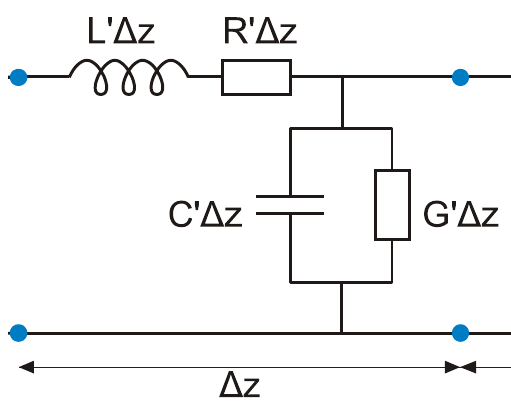
\includegraphics[width=.18\paperheight]{content/fuw/pictures/fuw_tem_ersatzschaltbild.png}
 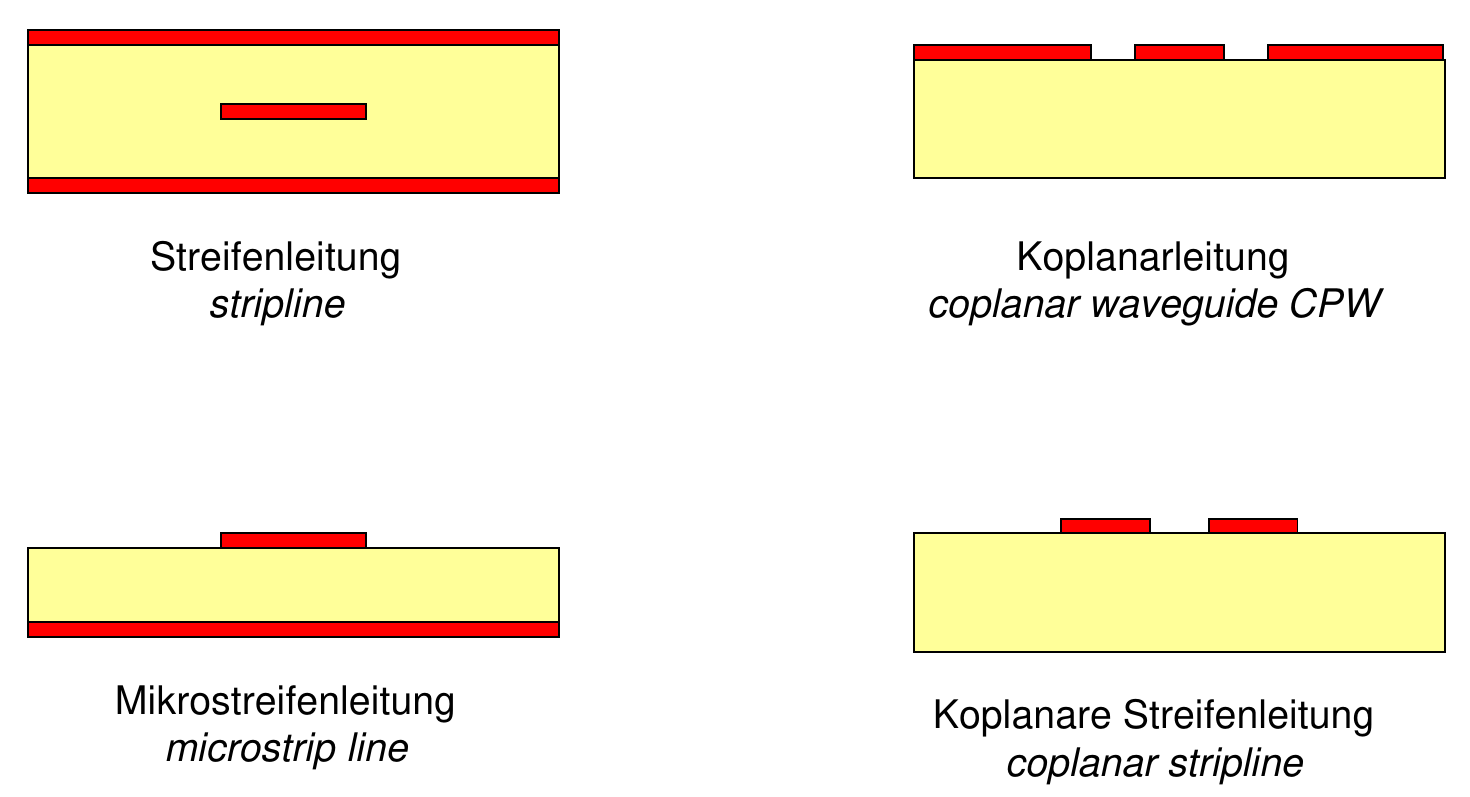
\includegraphics[width=.22\paperheight]{content/fuw/pictures/fuw_tem_leitungen.png}
  \begin{itemize}
     \itemsep0pt
     \item \textit{quasi-TEM} (\(\beta = \sqrt{\epsilon_{r,\mathrm{eff}}} k_0 \neq \sqrt{\epsilon_r} k_0\))
     \item Kapazitätsbelag mit ($C^\prime$) und ohne ($C_a^\prime, \epsilon_r = 1$) Dielektrikum
     \item \(\beta = \sqrt{\dfrac{C^\prime}{C_a^\prime}} = \sqrt{\epsilon_{r,\mathrm{eff}}} k_0\)
     \item Impedanzbereich eingeschränkt; typ. \SI{20}{\Omega}-\SI{300}{\Omega}
     \item \textbf{Berechnung der Kapazitätsbeläge:} entweder numerisch oder analytisch mit konforme Abbildung
     \item \textbf{Streifenleitung} $\implies$ echte TEM-Welle, \(\epsilon_r = \epsilon_{r,\mathrm{eff}}\)
     \item \textbf{Mikrostreifenleitung} $\implies$ einfache Fertigung, verlustarm, messtechnisch ungünstig
     \item \textbf{Koplanarleitung} $\implies$ messtechnisch günstig, serien-/parallelelemente leich integrierbar, mittlere Verluste, zwei Moden
     \item \textbf{Koplanare Streifenleitung}: symmetrisch, Leitungstranformer und Speiseleitung für Antennen 
     %\item Es existieren immer zwei unabhängige Lösungen, die den beiden möglichen Transportrichtungen entsprechen
     %\item \textit{Ausbreitungsgeschwindigkeit} und \textit{Impedanz} sind für beide Lösungen und an allen Orten der Leitung gleich und ausschließlich durch die Leitungsgeometrie und die Materialien festgelegt
     %\item Sämtliche Leitungseigentschaften lassen sich durch eine (quasi-)statische Analyse ermitteln (Kapazitätsbelag $C^\prime$ und Induktivitätsbelag $L\prime$ sind auch für Gleichstrom definiert!)
     \item Ausbreitungsgeschwindigkeit: \(c = \dfrac{1}{\sqrt{L^\prime C^\prime}}\)
 \end{itemize}
 \subsection{Planare Leitungen}
 }

        \vspace{1cm}
{\small%
\section{Zwei und Mehrtore}
\subsection{Komplexe Wellenamplituden}
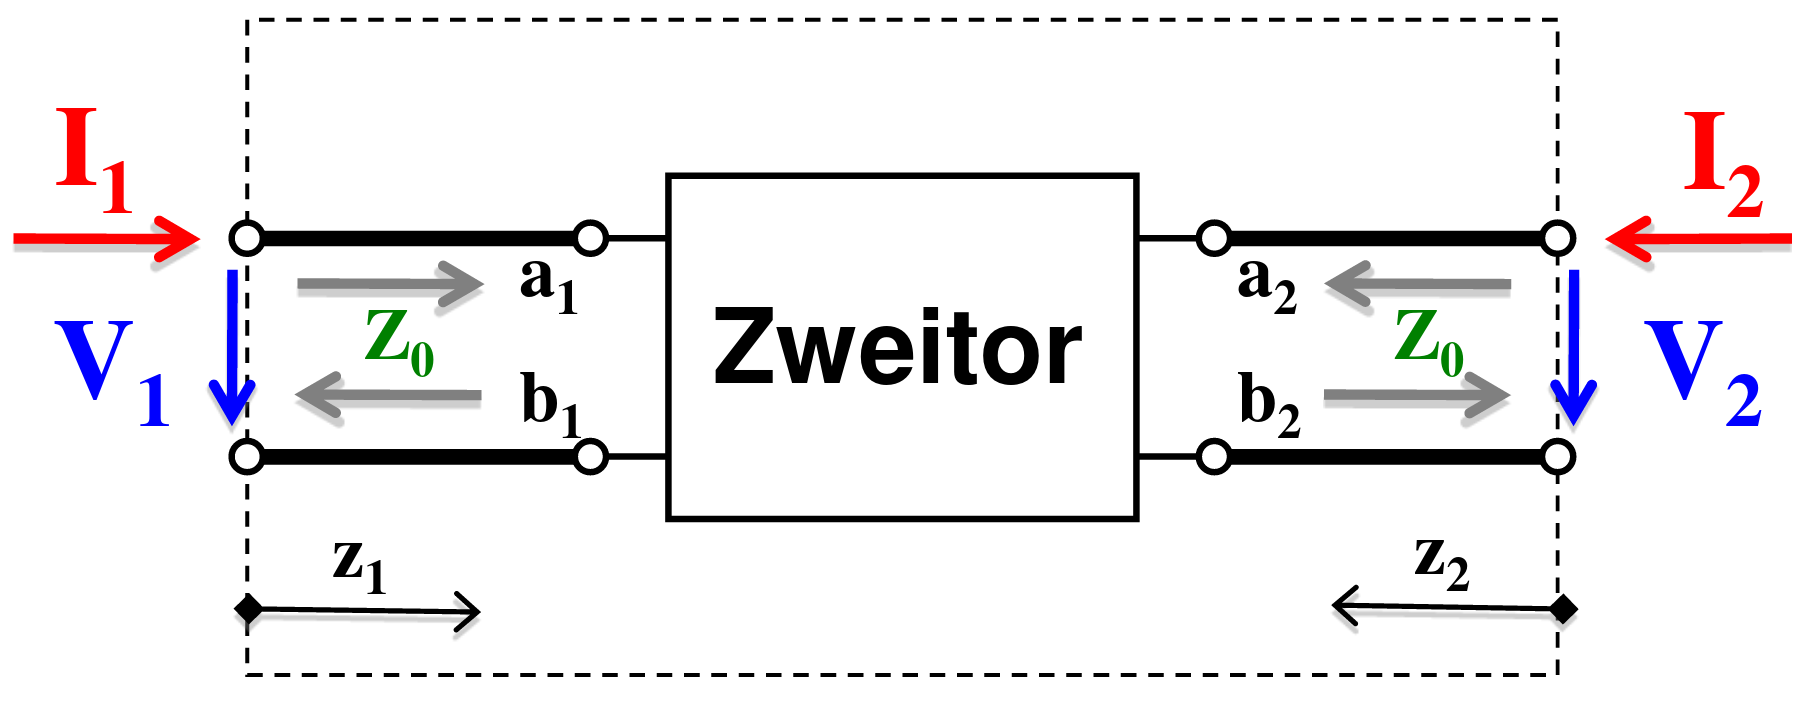
\includegraphics[width= 0.35\paperheight]{content/fuw/pictures/hf_zweitor.png}
    \begin{itemize}
        \itemsep0pt
        \item Verwendung von Strom/Spannung wenig sinnvoll, wegen der starken Empfindlichkeit zur Leitungslänge
        \item \textit{Stattdessen:} komplexe Amplituden $a$ und $b$
        \item Hinlaufende Welle $a_1$ bzw. $a_2$
        \item Rücklaufende Welle $b_1$ bzw. $b_2$
        \item Definition der Wellenamplituden:
        \begin{align*}
            a_k  = \dfrac{1}{2\sqrt{2 Z_0}}(U_k + Z_0 I_k)\\
            b_k  = \dfrac{1}{2\sqrt{2 Z_0}}(U_k - Z_0 I_k)
        \end{align*}
\end{itemize}
\subsection{Streuparameter}
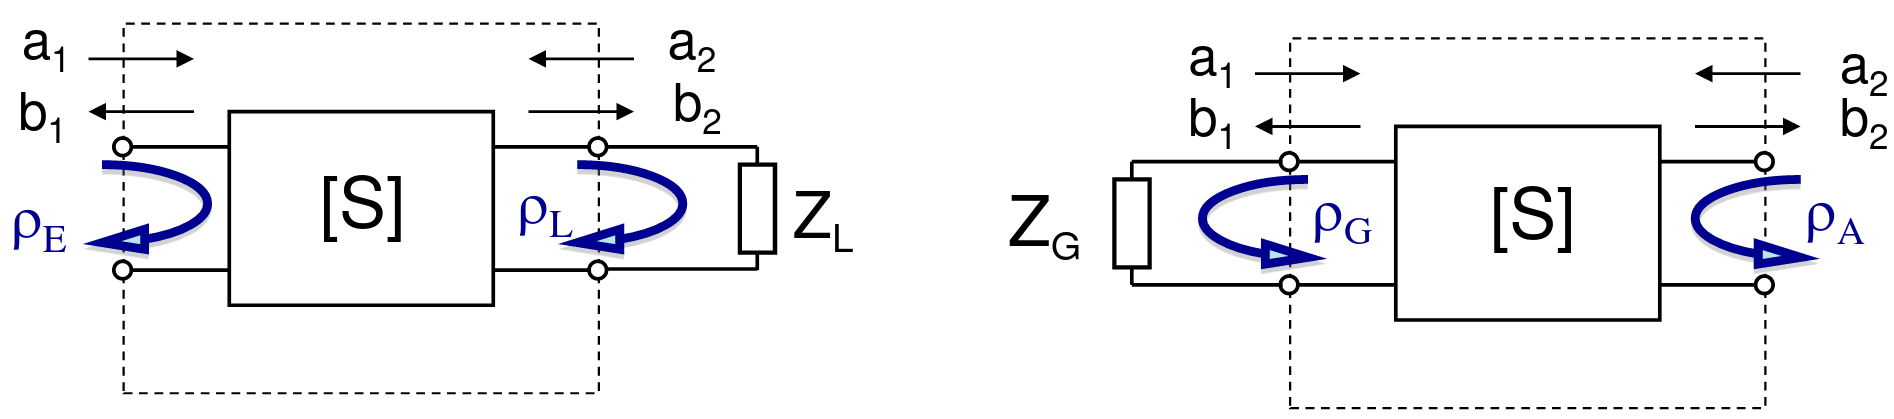
\includegraphics[width=0.35\paperheight]{content/fuw/pictures/hf_zweitor_reflektion.png}
\begin{itemize}
    \itemsep0pt
    \item Streuparameter der $S$-Matrix
    \item \textit{Allgemein:} \(\underline{b} = S \underline{a}\)
    \item Für ein Zweitor:
    \begin{align*}
        b_1 &= S_{11} a_1 + S_{12} a_2\\
        b_2 &= S_{21} a_1 + S_{22} a_2
    \end{align*}
    \item \textbf{Anpassung:} allseits reflexionsfrei\\
        \(s_{ii} = 0, \;\forall i \in (1;\; \mathrm{dim}(S))\)
    \item Eingangsreflexionsfaktor\\
        \(\rho_E = \dfrac{b_1}{a_1}; \;\;\; \rho_L = \dfrac{a_2}{b_2}\)
    \item Ausgangsreflexionsfaktor\\
        \(\rho_A = \dfrac{b_2}{a_2}; \;\;\; \rho_G = \dfrac{a_1}{b_1}\)
        \begin{align*}
            |\rho_E| = \left|S_{11} + \dfrac{S_{21} S_{12} \rho_L}{1 - S_{22} \rho_L}\right|\\
            |\rho_A| = \left|S_{22} + \dfrac{S_{12} S_{21} \rho_G}{1 - S_{11} \rho_G}\right|
        \end{align*}
    \item \textbf{Reziprozität} (Übertragungssymmetrie): \(S = S^\top\)
    \item \textbf{Verlustfreie} n-Tore ($S$ unitär):\\
        \(\sum^n_{i=1} |b_i|^2 = \sum^n_{i=1} |a_i|^2 \implies S^\top S^* = I\)
    \item Verlustfreies, reziprokes, allseits angepasstes 3-Tor\\
        \(\implies\) nicht realisierbar
\end{itemize}
\subsection{Alternative Netzwerkdarstellungen}
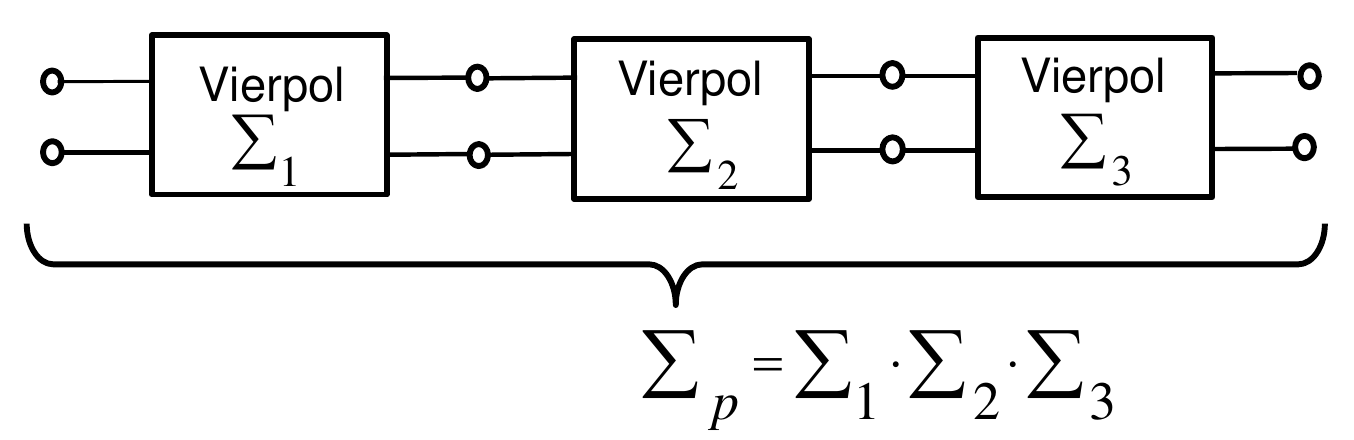
\includegraphics[width=0.35\paperheight]{content/fuw/pictures/fuw_transmissionsmatrix.png}
\begin{itemize}
    \itemsep0pt
    \item \textbf{Wellentransmissionsmatrix} $\Sigma$:\\
        \[\begin{bmatrix}b_1\\ a_1\end{bmatrix} = \begin{bmatrix}\Sigma_{11} & \Sigma_{12}\\ \Sigma_{21} & \Sigma_{22}\end{bmatrix} \begin{bmatrix}a_2\\ b_2\end{bmatrix}\]\\
    \item Streumatrix $\to$ Transmissionsmatrix
        \begin{align*}
            \Sigma_{11} &= -\dfrac{\Delta_S}{S_{21}} &\Sigma_{12} = \dfrac{S_{11}}{S_{21}}\\
            \Sigma_{21} &= -\dfrac{S_{22}}{S_{21}} &\Sigma_{22} = \dfrac{1}{S_{21}}
        \end{align*}
    \item \textbf{Ketten- bzw. ABCD-Matrix}:
        \[\begin{bmatrix}u_1\\ i_1\end{bmatrix} = \begin{bmatrix}A & B\\ C & D\end{bmatrix} \begin{bmatrix}u_2\\ -i_2\end{bmatrix}\]
        \item  $u$ und $i$ sind normierte Spannungen und Ströme:\\
            \(u = \dfrac{U}{\sqrt{Z_0}}; \;\; i = I\sqrt{Z_0}\)
        \item ABCD $\to$ Streumatrix:
            \begin{align*}
                S_{11} &= \dfrac{A+B-C-D}{A+B+C+D}, &S_{12} = \dfrac{2\:\mathrm{det}(ABCD)}{A+B+C+D},\\
                S_{21} &= \dfrac{2}{A+B+C+D}, &S_{22} = \dfrac{-A+B-C+D}{A+B+C+D}
            \end{align*}
        \item Streumatrix $\to$ ABCD:
            \begin{align*}
                A &= \dfrac{-\Delta_S + S_{11} - S_{22} + 1}{2 S_{21}},\\
                B &= \dfrac{\Delta_S + S_{11} + S_{22} + 1}{A+B+C+D},\\
                C &= \dfrac{\Delta_S - S_{11} - S_{22} + 1}{2 S_{21}},\\
                D &= \dfrac{-\Delta_S - S_{11} S_{22} + 1}{2 S_{21}}
            \end{align*}
        \item Längwiderstand bzw. Querleitwert mit Bezugswiderstand $Z_0$:\\
            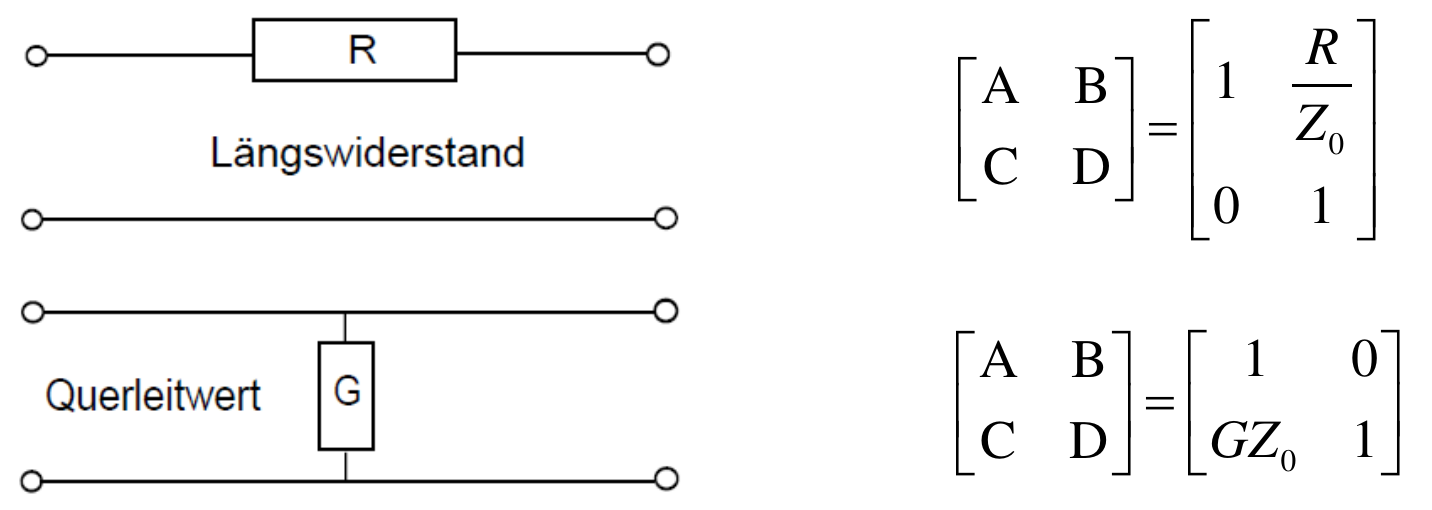
\includegraphics[width=0.35\paperheight]{content/fuw/pictures/fuw_kettenmatrix_widerstand_leitwert.png}
        \item Verlustlose Leitung (Wellenwiderstand $Z_l$, elektrische Länge $\beta l$, geometrische Länge $l$):
                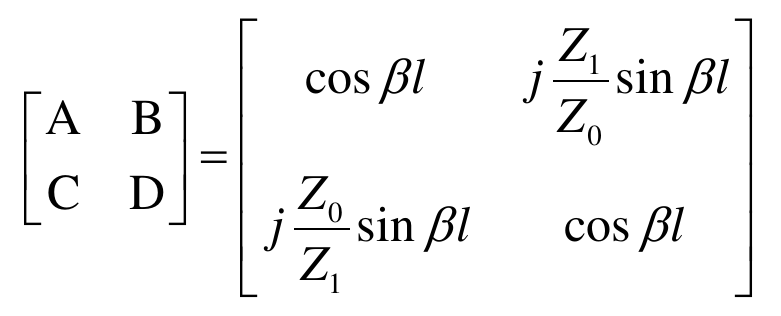
\includegraphics[width=0.28\paperheight]{content/fuw/pictures/fuw_kettenmatrix_leitung.png}
\end{itemize}
\subsection{Betriebsverhalten von Zweitoren}
\subsubsection{Zweitorverstärkung}
\begin{itemize}
    \itemsep3pt
    \item Die Übertragungsleistungsverstärkung (Gewinn $G$) ist die Ausgangsleistung bezogen auf die verfügbare Generatorleistung
    \item \(G = \dfrac{1 - |\rho_G|^2}{|1 - \rho_G \rho_E|^2} \cdot |s_{21}|^2 \cdot \dfrac{1 - |\rho_L|^2}{|1 - \rho_{L}s_{22}|^2}\)
    \item Bei Rückwirkungsfreiheit $s_{12} = 0$ ($\rho_E = s_{11}$):\\
        \(G = \dfrac{1 - |\rho_G|^2}{|1 - \rho_G s_{11}|^2} \cdot |s_{21}|^2 \cdot \dfrac{1 - |\rho_L|^2}{|1 - \rho_{L}s_{22}|^2}\)
    \item \textit{Daumenregel für Rückwirkungsfreiheit}: \(\dfrac{S_{12}}{S_{21}} \ll 1 \implies \dfrac{S_{12}}{S_{21}} \leq 0.1\)
    \item Maximale (unilaterale für $s_{12} = 0$) Leistungsverstärkung:\\
        \(G_{max} = \dfrac{|s_{21}^2|}{(1 - |s_{11}|^2) (1 - |s_{22}^2|)}\)
\end{itemize}
\subsubsection{Verstärker mit Anpassnetzwerken}
\begin{itemize}
    \itemsep0pt
    \item Max. Leistungsverstärkung erfordert Wirkleistungsanpassung am Ein- und Ausgang
    \item Hochfrequenzverstärker (Transistoren) weisen stark reaktive u. frequenzveränderliche Impedanz auf
    \item Diese muss durch geeignete reaktive Netzwerke angepasst werden
    \item Probleme:\vspace{-.5cm}
        \begin{itemize}
            \itemsep0pt
            \item Reaktive Anpassung $\to$ schmalbandig
            \item Reflexionen zwischen Verstärker und Anpassnetzwerk $\to$ Stabilitätsprobleme
        \end{itemize}
    \item \textbf{Absolute Stablilität:} Die Tore verhalten sich, unabhängig von der Beschaltung, \textit{passiv} $\implies$ \(\left(\mathrm{Re}\{Z_E\} > 0\right) \:\wedge\: \left(\mathrm{Re}\{Z_A\} > 0\right)\)
    \item \textbf{Bedingungen für Absolute Stabilität}:
    \begin{align*}
        &|S_{11}| < 1, &|S_{12} \cdot S_{21}| < 1 - |S_{22}|^2,\\
        &|S_{22}| < 1, &|S_{12} \cdot S_{21}| < 1 - |S_{11}|^2,\\
        %&K > 1; &K = \dfrac{1 + |\Delta_S|^2 - |S_{11}|^2 - |S_{22}|^2}{|2\, S_{12} S_{21}|}
    \end{align*}
        \(K = \dfrac{1 + |\Delta_S|^2 - |S_{11}|^2 - |S_{22}|^2}{|2\, S_{12} S_{21}|} > 1\)
    \item \textbf{Stabilitätskreise} für den Ein- ($C_L$, $R_L$) bzw Ausgang ($C_G$, $R_G$):
        \begin{align*}
            &C_L = \dfrac{\left(S_{22} - \Delta_S S_{11}^*\right)^*}{|S_{22}|^2 - |\Delta_S|^2},\
            &R_L = \left|\dfrac{S_{12} S_{21}}{|S_{22}|^2 - |\Delta_S|^2}\right|,\\
            &C_G = \dfrac{\left(S_{11} - \Delta_S S_{22}^*\right)^*}{|S_{11}|^2 - |\Delta_S|^2},\
            &R_G = \left|\dfrac{S_{12} S_{21}}{|S_{11}|^2 - |\Delta_S|^2}\right|,
        \end{align*}
\end{itemize}
\subsection{Gebräuchliche Mehrtorschaltungen}
\subsubsection{Leitungskoppler, Reflektometerschaltung}
\begin{itemize}
    \itemsep0pt
    \item Dienen dazu hin- und rücklaufenden Wellen a \& b zu trennen
    \item \textbf{Bauelemente zur Trennung der Welle:} \textit{Richtkoppler}
\end{itemize}
}

        \section{Theoreme der Feldtheorie}
\subsection{Elektromagnetische Energiebilanz}
\begin{itemize}
    \itemsep0pt
    \item \textbf{PEC} (\textit{perfectly electrically conducting}): \(E_{tan} = \vec{n} \times \vec{E} = 0\)
    \item Komplexe Poynting-Vektor: \(\vec{S} = \dfrac{1}{2} \vec{E} \times \vec{H}^*\)
    \item Gesamte Verlustleistung: \(P_V = P_\kappa + P_\epsilon + P_\mu\)
    \item Zeitharmonische Vorgänge in einem abgeschlossenen, quellenfreien Gebiet:\\
        \[\oiint\limits_{A(V)}\vec{S}\cdot\mathrm{d}\vec{A} = - P_V + 2j\omega\,(\overline{W}_e - \overline{W}_m)\]
\end{itemize}
\subsection{Reziprozität}
\begin{itemize}
    \item \textbf{Allgemeine Form des Reziprozitätstheorems:}\\
        \begin{align*}
            &\iiint\limits_V\left(\vec{E}_1 \cdot \vec{J}_2 - \vec{H}_1 \cdot \vec{M}_2\right)\mathrm{d}v\\
            &= \iiint\limits_V\left(\vec{E}_2 \cdot \vec{J}_1 - \vec{H}_2 \cdot \vec{M}_1\right)\mathrm{d}v
        \end{align*}
\end{itemize}
\subsection{Elektromagnetische Potentiale}
\begin{itemize}
    \itemsep1pt
    \item Magnetische Vektorpotential \(\vec{B} = \nabla\times\vec{A}\)
    \item \textit{Helmholtz-Theorem} besagt, dass jede beliebige Vektorfeld im freien Raum geschrieben werden kann als:\\
        \(\vec{A} = \nabla\times\vec{C} + \nabla\xi\)
    \item Freiheitsgrad: \(\vec{B} = \nabla\times\vec{A} = \nabla\times\nabla\times\vec{C}\)
    \item Elektrische Skalarpotential $\varphi$:\\
        \(\vec{E} = -j\omega\vec{A} - \nabla\varphi\)
    \item \textbf{Vektorielle Helmholz-Gleichung:}\\
        \(\Delta\vec{A} + k^2\vec{A}  = -\mu\vec{J}\)
    \item \textbf{Skalare Helmholz-Gleichung:}\\
        \(\Delta\varphi + k^2\varphi = -\dfrac{\rho}{\epsilon}\)
    \item \textbf{Analog:} elektrische Vektorpotential $\vec{F}$ und skalare magnetische Potential $\psi$
        \begin{align*}
            \vec{D} &= -\nabla \times \vec{F}\\
            \vec{H} &= -j\omega\vec{F} - \nabla\psi
        \end{align*}
\end{itemize}
\subsection{Green'sche Funktionen}
\begin{itemize}
    \itemsep1pt
    \item Verhält sich wie ein \textit{Impulsantwort} der Feldlösung einer bestimmten Geometrie
    \item Poisson-Gleichung: \(\Delta G^\varphi(\vec{r}, \vec{r}^\prime) = -\dfrac{1}{\epsilon}\delta(\vec{r}, \vec{r}^\prime)\)
    \item Sind die Feldgrößen \textit{Skalare}, so ist die Green'sche Funktion ein \textit{Skalar}\\
        $\implies$ $\rho$ und $\varphi$ sind Skalare, also ist $G^\varphi$ ein Skalarfeld
    \item Sind die Feldgrößen \textit{Vektoren}, so ist die Green'sche Funktion eine \textit{Dyade}\\
        $\implies$ $\vec{J}$ und $\vec{A}$ sind Vektoren, also ist $\dyade{G}^A$ eine Dyade
        \begin{align*}
            \vec{A} &= \iiint\limits_V \dyade{G}^A(\vec{r},\vec{r}^\prime) \cdot \vec{J}(\vec{r}^\prime)\:\mathrm{d}v^\prime =\\
            &= \iiint\limits_V\
            \begin{pmatrix}\
                G^A_{xx}(\vec{r},\vec{r}^\prime) & G^A_{xy}(\cdot) & G^A_{xz}(\cdot)\\
                G^A_{yx}(\cdot) & G^A_{yy}(\cdot) & G^A_{yz}(\cdot)\\
                G^A_{zx}(\cdot) & G^A_{zy}(\cdot) & G^A_{zz}(\cdot)
            \end{pmatrix}\
            \begin{pmatrix}\
                J_x(\vec{r}^\prime)\\
                J_y(\vec{r}^\prime)\\
                J_z(\vec{r}^\prime)
            \end{pmatrix}\
            \mathrm{d}v^\prime
        \end{align*}
    \item Green'sche Funktionen \textbf{des freien Raumes:}\\
        \begin{align*}
            &G(\vec{r},\vec{r}^\prime) = \dfrac{\mathrm{e}^{-jk\:|\vec{r} - \vec{r}^\prime|}}{4\pi|\vec{r} - \vec{r}^\prime|},\\
            &\dyade{G}^A(\vec{r},\vec{r}^\prime) = \mu\dfrac{\mathrm{e}^{-jk\:|\vec{r} - \vec{r}^\prime|}}{4\pi|\vec{r} - \vec{r}^\prime|}\dyade{I},\\
            &\dyade{G}^F(\vec{r},\vec{r}^\prime) = \epsilon\dfrac{\mathrm{e}^{-jk\:|\vec{r} - \vec{r}^\prime|}}{4\pi|\vec{r} - \vec{r}^\prime|}\dyade{I}
        \end{align*}
    \item Green'sche Funktionen des freien Raumes, bei \textbf{Anregung mit elektrischen Strömen:}\\
        \begin{align*}
            &\dyade{G}^E_J(\vec{r},\vec{r}^\prime) = -j\omega\mu\left[\left(\dyade{I} + \dfrac{1}{k^2}\nabla\nabla\right) \dfrac{\mathrm{e}^{-jk\:|\vec{r} - \vec{r}^\prime|}}{4\pi|\vec{r} - \vec{r}^\prime|}\right]\\
            &\dyade{G}^H_J(\vec{r},\vec{r}^\prime) = \nabla\;\dfrac{\mathrm{e}^{-jk\:|\vec{r} - \vec{r}^\prime|}}{4\pi|\vec{r} - \vec{r}^\prime|} \times \dyade{I}\\
        \end{align*}
    \item Green'sche Funktionen des freien Raumes, bei \textbf{Anregung mit magnetischen Strömen:}\\
        \begin{align*}
            &\dyade{G}^E_M(\vec{r},\vec{r}^\prime) = -\nabla\;\dfrac{\mathrm{e}^{-jk\:|\vec{r} - \vec{r}^\prime|}}{4\pi|\vec{r} - \vec{r}^\prime|} \times \dyade{I}\\
            &\dyade{G}^H_M(\vec{r},\vec{r}^\prime) = -j\omega\epsilon\left[\left(\dyade{I} + \dfrac{1}{k^2}\nabla\nabla\right) \dfrac{\mathrm{e}^{-jk\:|\vec{r} - \vec{r}^\prime|}}{4\pi|\vec{r} - \vec{r}^\prime|}\right]\\
        \end{align*}

\end{itemize}
\subsection{Spiegelungsprinzip}
\subsection{Huygen'sches Prinzip}

        \vspace{1cm}
\section{Leitungsgeführte EM-Wellen}
\subsection{Feldtypen im homogenen zylindrischen Wellenleiter}
\begin{itemize}
    \itemsep0pt
    \item Nicht zwingend kreiszylindrisch!
    \item Translationsinvarianz des Wellenleiters in z-Richtung
    \item Ausbreitungskoeffizient $\gamma$:
        \begin{itemize}
            \itemsep0pt
            \item Sich ausbreitende Welle:\\
                \(\gamma = 0 + j\beta,\; q \leq k\)
            \item Evaneszente (gedämpfte) Welle:\\
                \(\gamma = \alpha + j0,\; q > k\)
            %\item Abklingende, sich ausbreitende, Welle: \(\gamma = \alpha + j\beta\)
        \end{itemize}
    \item Modenspezifischer, geometrieabhängiger Eigenwert \(q\):\\
        \(|k|^2 = k_x^2 + k_y^2 + k_z^2 = q^2 + k_z^2,\: k = \omega_c \sqrt{\mu\epsilon}\)
    \item Ausbreitung \textit{nur} oberhalb der Cut-off-Frequenz \(f_c\) bzw. \(\omega_c\) \(\implies k_z = 0\)\\
    \item Feldwellen(typ)-Widerstände:
        \begin{align*}
            Z_{FH} &= \dfrac{j\omega\mu}{\gamma_H} = \dfrac{\omega\mu}{\beta_H} = \dfrac{\lambda_g}{\lambda_{HEW}}Z_{F}\\
            Z_{FE} &= \dfrac{j\omega\mu}{\gamma_E} = \dfrac{\beta_E}{\omega\epsilon} = \dfrac{\lambda_g}{\lambda_{HEW}}Z_{F}\\
            \lambda_g &= \dfrac{2\pi}{\beta} = \dfrac{2\pi}{\sqrt{\omega^2\epsilon\mu - q^2}},\
            Z_F = \sqrt{\dfrac{\mu}{\epsilon}}
        \end{align*}
\end{itemize}
\subsection{Phasen- und Gruppen-Geschwindigkeit}
\begin{itemize}
    \itemsep0pt
    \item Phasengeschwindigkeit: \(v_p = \dfrac{\omega}{\beta}\)
    \item (Gruppen-)Geschwindigkeit der informationstragenden Hüllkurve:\\
        \(v_g = \left( \dfrac{\mathrm{d}\beta}{\mathrm{d}\omega} \right)^{-1}\)
    \item \(\dfrac{v_p}{c_0} =  \dfrac{\lambda_g}{\lambda_0} = \dfrac{Z_{FH}}{Z_0} =\
        \left(\dfrac{v_g}{c_0}\right)^{-1} = \left(\dfrac{Z_{FE}}{Z_0}\right)^{-1} = \dfrac{k}{k_z}\)
\end{itemize}
\subsection{Fünf-Komponenten-Felder (E- und H-Moden)}
\begin{itemize}
    \itemsep0pt
    \item \textbf{Ansatz:} Im zylind. Wellenleiter, können transversale und longitudinale Felder getrennt betrachtet werden
    \item \((u,v)\) sind beliebige krummlinige Koordinaten:
        \begin{align*}
            \vec{E}(u, v, z) &= \left[ \vec{E}_t(u,v) + \vec{e}_z E_z \right]\mathrm{e}^{-\gamma z}\\
            \vec{H}(u, v, z) &= \left[ \vec{H}_t(u,v) + \vec{e}_z H_z \right]\mathrm{e}^{-\gamma z}
        \end{align*}
    \item Die Kenntnis der z-Komponente reicht, um die restlichen 4 Komponenten zu berechnen
\end{itemize}
\subsection{Rechteckhohlleiter}
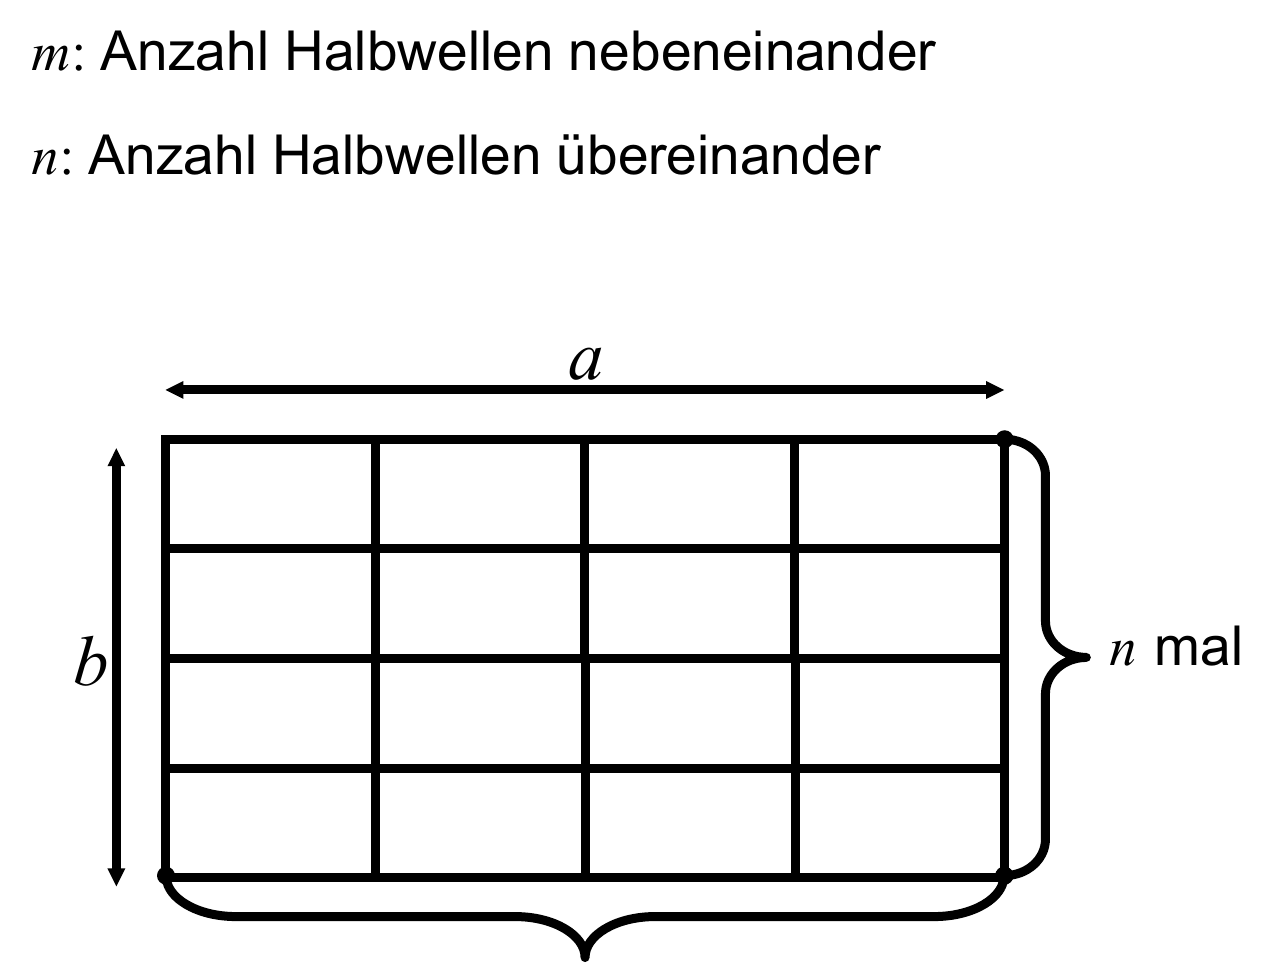
\includegraphics[width=.35\paperheight]{content/fuw/pictures/fuw_rechteckhohlleiter.png}
\begin{itemize}
    \itemsep0pt
    \item \(E_{mn}\) (TM)-Moden/Feldtypen im Rechteckhohlleiter \(H_z = 0\):
        \begin{align*}
            E_z &= E_0 \sin\left(\dfrac{m\pi x}{a}\right)\sin\left(\dfrac{n\pi y}{b}\right)\mathrm{e}^{-j\beta z},\\
            E_y &= -j\dfrac{\beta}{\beta_c^2} \dfrac{m\pi}{a}  E_0\cos\left(\dfrac{m\pi x}{a}\right)\sin\left(\dfrac{n\pi y}{b}\right)\mathrm{e}^{-j\beta z},\\
            E_x &= j\dfrac{\beta}{\beta_c^2} \dfrac{n\pi}{b} E_0 \sin\left(\dfrac{m\pi x}{a}\right)\cos\left(\dfrac{n\pi y}{b}\right)\mathrm{e}^{-j\beta z},\\
            H_y &= -H_x Z_{FH},\\
            H_x &= H_y Z_{FH}
        \end{align*}
    \item \(H_{mn}\) (TE)-Moden/Feldtypen im Rechteckhohlleiter \(E_z = 0\):
        \begin{align*}
            H_z &= H_0 \cos\left(\dfrac{m\pi x}{a}\right)\cos\left(\dfrac{n\pi y}{b}\right)\mathrm{e}^{-j\beta z},\\
            H_y &= j\dfrac{\beta}{\beta_c^2} \dfrac{n\pi}{b}  H_0 \cos\left(\dfrac{m\pi x}{a}\right)\sin\left(\dfrac{n\pi y}{b}\right)\mathrm{e}^{-j\beta z},\\
            H_x &= j\dfrac{\beta}{\beta_c^2} \dfrac{m\pi}{a} H_0 \sin\left(\dfrac{m\pi x}{a}\right)\cos\left(\dfrac{n\pi y}{b}\right)\mathrm{e}^{-j\beta z},\\
            E_y &= -\dfrac{E_y}{Z_{FE}},\\
            E_x &= \dfrac{E_x}{Z_{FE}}
        \end{align*}
    \item Cut-off-Wellenlänge: \(\lambda_c = \dfrac{1}{\sqrt{ \left(\dfrac{m}{2a}\right)^2 + \left(\dfrac{n}{2b}\right)^2 }}\)
    \item \(\beta_c = \dfrac{2\pi}{\lambda_c}\)
\end{itemize}
%\begin{itemize}
%    \item Verlustleistung:
%        \begin{align*}
%            \Delta P_1 &= -\dfrac{1}{4}R_{\Box}a\dfrac{|E_0|^2}{|Z_{FH}|^2}\Delta z\\
%            \Delta P_2 &= -\dfrac{1}{4}R_{\Box}a\dfrac{|E_0|^2}{|Z_{F0}|^2} \left(\dfrac{\lambda_0}{2a}\right)^2 \Delta z\\
%            \Delta P_3 &= \dfrac{1}{2}R_{\Box}b\dfrac{|E_0|^2}{|Z_{F0}|^2} \left(\dfrac{\lambda_0}{2a}\right)^2 \Delta z
%        \end{align*}
%    \item Dämpfungskonstante: \[\alpha = \dfrac{R_{\Box}}{Z_{F0}} \dfrac{\frac{1}{b} + \frac{2}{a} \left(\frac{\lambda_0}{2a}\right)^2}{\sqrt{1 - \left(\frac{\lambda_0}{2a}\right)^2}}\
%        \]
%\end{itemize}
\subsection{Hohlleiter unterhalb der kritischen Frequenz}
\textbf{Exponentielle Dämpfung}
\[\alpha = \dfrac{2\pi}{\lambda_{HEW}} \sqrt{\left(\dfrac{\lambda_{HEW}}{\lambda_c}\right)^2 - 1}\
= \dfrac{2\pi}{\lambda_c} \sqrt{1 - \left(\frac{f}{f_c}\right)^2}\]
\subsection{Dielektrische Wellenleiter}


        \vspace{1cm}
\section{Strahlungsfelder und Antennen}
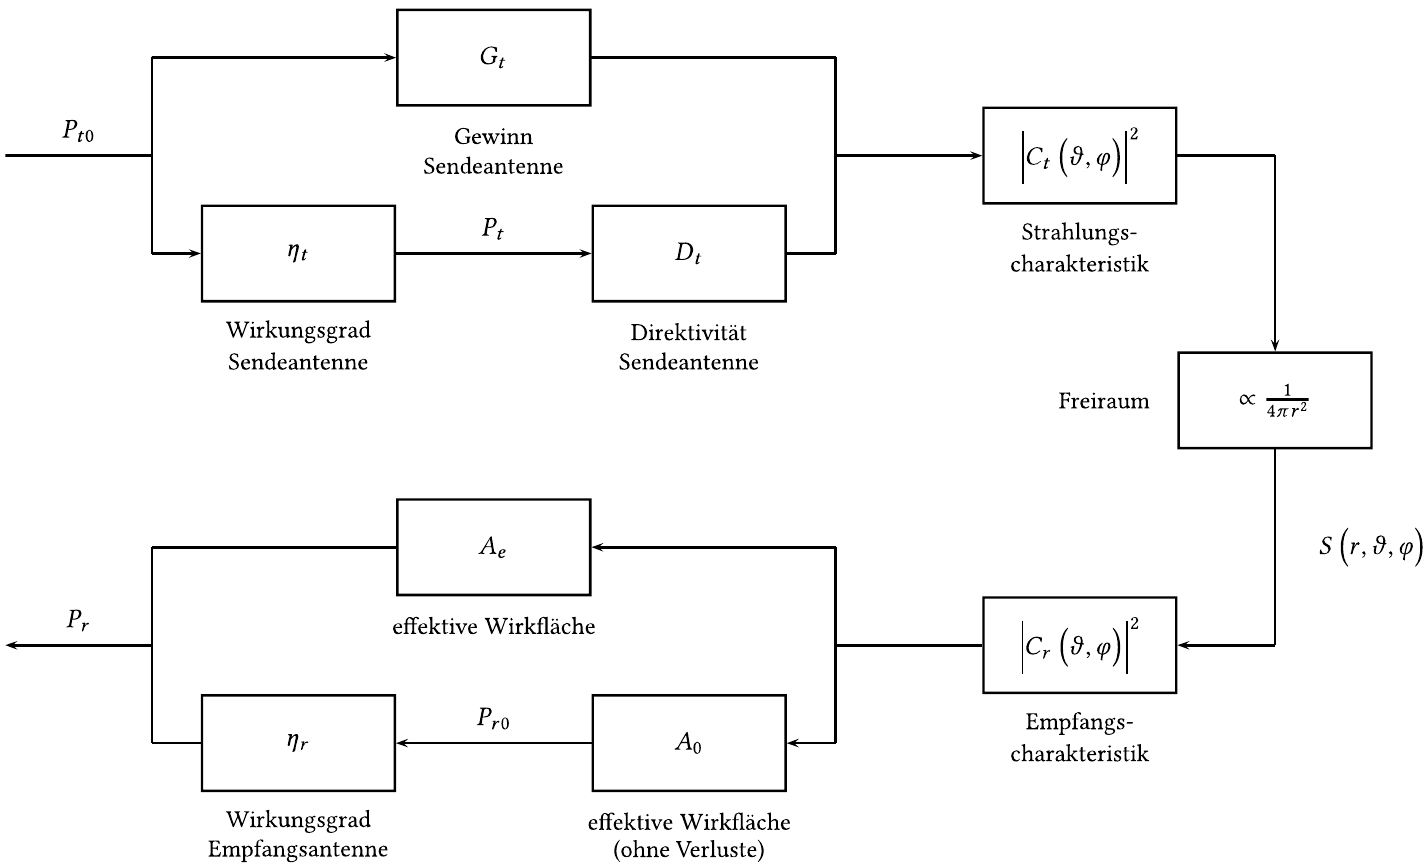
\includegraphics[width=.4\paperheight]{content/fuw/pictures/fuw_antenne.png}
\begin{itemize}
    \itemsep0pt
    \item Effektive Wirkfläche \(A_e = \dfrac{\lambda^2}{\pi} G_r\)
    \item Sendeantenne optimal ausgerichtet:\\
        \(\left|C_r(\vartheta, \varphi)\right| = 1 \implies S(r,\vartheta,\varphi) = S_{\mathrm{max}}(r)\)
    \item Empfangsantenne optimal ausgerichtet:\\
        \(\left|C_r(\vartheta, \varphi)\right| = 1 \implies P_r = P_{r, \mathrm{max}}\)
    \item \textbf{Fernfeld:} \(r \gg \lambda \implies kr \gg 2\pi\)
    \item Senden:
        \begin{itemize}
            \itemsep0pt
            \item Gesendete Leistung (ohne Verluste) \(P_{t0}\)
            \item Gesendete Leistung \(P_t\)
            \item Leistungsflussdichte \(S(r, \vartheta, \varphi)\)
            \item Leistungsflussdichte (\textit{isotroper Kugelstrahler}) \(S_i(r) = \dfrac{P}{4\pi r^2}\)
            \item Strahlungscharakteristik \(C_t(\vartheta, \varphi) = \left.\dfrac{E(\vartheta, \varphi)}{E_{max}}\right|_{r = \mathrm{const}}\)
            \item Direktivität \(\left.D_t = \dfrac{S_{max}}{S_i}\right|_{P_t} = \dfrac{4\pi r^2 S_{max}}{P_{t}}\)
            \item Gewinn \(\left.G_t = \dfrac{S_{max}}{S_i}\right|_{P_{t0}} = \dfrac{4\pi r^2 S_{max}}{P_{t0}}\)
            \item Wirkungsgrad \(\eta_t = \dfrac{G_t}{D_t}\)
        \end{itemize}
    \item Empfangen:
        \begin{itemize}
            \itemsep0pt
            \item Empfangene Leistung (ohne Verluste) \(P_{r0}\)
            \item Empfangene Leistung \(P_r\)
            \item Empfangscharakteristik \(C_r(\vartheta, \varphi) = \left.\dfrac{U(\vartheta, \varphi)}{U_{max}}\right|_{S = \mathrm{const}}\)
            \item Effektive  Wirkfläche (ohne Verluste): \(A_0 = \dfrac{P_{r0,\mathrm{max}}}{S} = \dfrac{\lambda^2}{4\pi}D_r\)
            \item Effektive  Wirkfläche: \(A_e = \dfrac{P_{r,\mathrm{max}}}{S} = \dfrac{\lambda^2}{4\pi}G_r\)
            \item Wirkungsgrad \(\eta_r = \dfrac{A_e}{A_0}\)
        \end{itemize}

\end{itemize}

        \section{Physikalische Konstanten}
        \begin{align*}
            c_0 &= \frac{1}{\sqrt{\mu_0\epsilon_0}} = \SI{3.0e8}{\frac{m}{s}}\\
            \mu_0 &= \SI{4\pi e-7}{\frac{Vs}{Am}}\\
            \epsilon_0 &= \SI{8.854e-12}{\frac{Vs}{Am}}\\
            Z_{F0} &= \sqrt{\frac{\mu_0}{\epsilon_0}} \approx \SI{377}{\Omega}
        \end{align*}
        \section{Notation}
        \centering
        \(\Delta_X \equiv \mathrm{det}(X)\)
    \end{multicols}
\end{document}
